Cell line development (CLD) is a process of generating single cell-derived clones that produce high and consistent levels of target therapeutic protein [TODO cite pharma.lonza.com/offerings/mammalian/cell-line-development]. Therapeutic proteins in this case are so-called recombinant proteins and they are widely used in the biomedical research, drug production and for various therapeutic needs like, for example, vaccines and monoclonal antibodies (mAbs) \cite[see]{IWNLP} \supercite{iqbal2007underwater} [TODO cite Ohtake 2013, Jefferis 2021, Funaro 1996]. A recombinant protein is defined by [cite Barbeau, J] is a modified or manipulated protein encoded by a recombinant DNA. Recombinant DNA, in its turn, consists of a plasmid, where the genes of the target protein of interest are cloned downstream of a promoter region. As soon as this plasmid will be transfected to a host cell (for example some mammalian cells that are able to produce the protein), the host will start to express this protein of interest. Today, in both industry and research there is a great need for production of high volumes of good-quality recombinant proteins [TODO cite Tihanyi 2020]. That is why the goal of many research efforts in recombinant protein production is to improve expression efficiency and create high-throughput systems to improve the CLD processes [cite Tihanyi 2020].


One of the most popular host cells used in CLD and in this work specifically are chinese hamster ovary (CHO) cells [cite Castan 2018]. Altough different cells can be used as hosts, such as bacterial, plant-based or yeast cells, mammalian cells remain the most popular [cite Beckman]. The reason behind this popularity hides in the fact that they can produce a diverse range of correctly folded proteins and most importantly, they have high protein production rates. Productivity rate is measured in titre of produced protein, and CHO cells can reach 0.1 - 1 g/L in batch and 1-10 g/L in fed-batch [TODO add reference] cultures [cite Tihanyi 2020]. Mostly all of the mAbs are produced using CHO cells [cite Lalonde 2017]. Companies mostly use the same host cell line for all their productions because already checked and qualified cells simplify the road to the clinic [cite Tihanyi 2020]. That is why current research has a wide applicability.

However there is a downside to using CHO as host cells - they are infamously unstable. As rapidly growing immortal cells CHO are also genomically unstable and extremely heterogeous which ususally leads to the main issue: production instability. The problem of choosing stable and high-production clones that simutaneously will be able to express protein qualitatively and quantifiably over time is essentially the main goal of current research. The big challenge in manufacturing here is the time and the costs of production. Currently, a lot of research attention is dedicated to the reduction of both, as well as to developing techniques of high-throughput clone screening and characterization [cite Tihanyi 2020]. The latter is of interest for this thesis. With the great amounts of data acquired over time and the development of the computational modelling and statistical analysis it is possible now to do the analysis \textit{in silico}, meaning - computationally without interferring with the cells instead of the usual \textit{in vitro} analysis.

\paragraph{CLD steps}
\begin{figure}[H]
	\begin{center}
		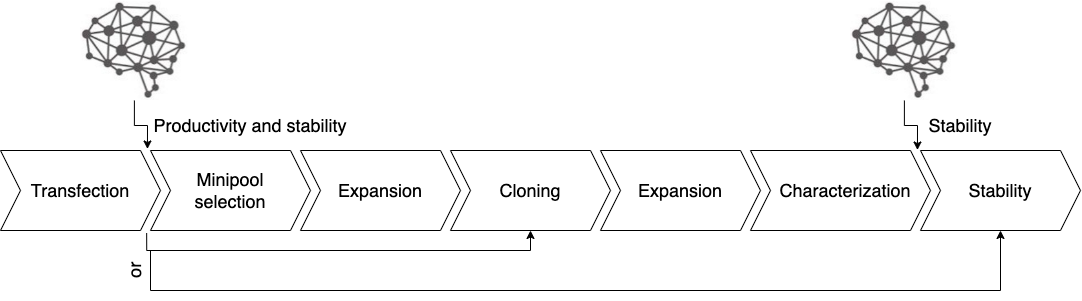
\includegraphics[width=0.8\linewidth]{bilder/CLD.png}
		\caption{CLD process steps}\label{fig:cls-steps}
	\end{center}
\end{figure}

The first step of CLD is called transfection - the introduction of the gene of interest (GOI or a DNA vector or alternatively an expression vector) into CHO cells. It has two main problems: first is that transfection mostly results in a vector being inserted into a random site within the host cell genome and second, that it generally has low efficiency of integration [cite Tihanyi]. It is important to transfect a GOI into the optimal site of the genome to secure high protein expression over time during protein production, however practically, transfection happens into a random location of genome. In cases where the gene was transfected into an inactive site of genome (essentially the majority of genome is transcriptionally inactive), the cell will likely be unable to express the gene [cite Castan, Hong 2018].

The second step of the process is selection of cell minipools that have successful and stable gene integrations for further expansion and cloning. The reason for not all of them being suitable is that during the transfection step, only 80\% of the cells will receive a GOI vector [cite Castan]. Only a small percent of these cells actually integrate a vector into the genome and, as mentioned above, only a fraction of those are able to stably express the protein [a better reference needed Shin 2020]. After the best minipools are selected, they will be expanded.

The third step in CLD is to clone the cells. Chosen stable pools of cells are phenotypically and genetically diverse - meaning they have different growth rates, metabolic profile and etc. This is not ideal for industrial production - all the cells used for protein production should be derived from the same clone [cite [25] from Castan]. 

Once the cells are cloned, phenotypical and genetical heterogeneity is reduced, the next step is to characterize the cells for their expression of the GOI. One has to estimate the clones' productivity and stability. Such observations may take up to 90 days (usually the checks are made on the 30th, 60th and 90th days). If the clones remain stable after this time and are able to express enough of the protein, then they are suitable for further production. However this last step costs a lot of time and maintenance costs for feeding and analysing the cells. Predicting productivity and stability of the cells on ealier stages would reduce this time significantly or even allow to avoid this process completely. 